\frame{\sectionpage}

 
 \begin{frame}{Topological recursion}
    \( \Sigma \) curve  inside \(\mathbb{C}^2\), with divisor \( R \). % one dimensional scheme
    
    Algorithm -- recursion in two non-negative integers \(g,n\). 

    Produces a collection of \emph{meromorphic}, \emph{symmetric} polydifferentials or invariants \(  \omega_{g,n}\) 
    \[ \omega_{g,n} \in \Gamma(  \left(\Sigma - R \right)^n, \kappa_\Sigma^{\boxtimes n} )   .\] 
    \begin{ex}
    \[ \omega_{0,1} = 2 z_1^2 dz_1 ,\quad  \omega_{0,2} = \frac{dz_1 \, dz_2}{(z_1^2 - z_2^2) }. \]
    \end{ex}
    
    Why do we care? \( \omega_{g,n}\) compute interesting numbers, string theory, enumerative geometry etc.
    \end{frame} 
    
    
    
    \begin{frame} 
    Initial conditions \( \omega_{0,3}\), \(\omega_{1,1}\) given.
    \begin{defn}[Topological recursion]
    \begin{align*}\omega_{g,n}(z_{\sbt}) =& \sum_{\alpha \in \text{Ram} } \Res_{z = \alpha}  K(z_1, z) \Big[ \omega_{g-1, n+1} (z, \sigma_\alpha(z), z_2, \dots, z_n) \\
    + &\sum_{\substack{g_1 + g_2 = g \\ I_1 \sqcup I_2 = \{z_2\dots,z_n\} }} \omega_{g_1, \# I_1+1}(z,I_1) \, \omega_{g_2, \#I_2  +1}(\sigma(z), I_2) \Big]
    \end{align*}
    \( \sigma \) local involution at ramification point, \( K(z_1,z)\) recursion kernel, \( z_{\sbt} = (z_1, \dots z_n)\).
    \end{defn} 
    Take away: Quadratic relations in \( \omega_{g,n}\). Could it look like relations from a conic?
    \end{frame}
    
    \begin{frame}
        \begin{center}
        

\tikzset{every picture/.style={line width=0.75pt}} %set default line width to 0.75pt        

\begin{tikzpicture}[x=0.75pt,y=0.75pt,yscale=0.8,xscale=0.8]
%uncomment if require: \path (0,475); %set diagram left start at 0, and has height of 475

%Shape: Ellipse [id:dp47766951388601575] 
\draw   (117.44,140) .. controls (117.44,134.48) and (119.68,130) .. (122.44,130) .. controls (125.2,130) and (127.44,134.48) .. (127.44,140) .. controls (127.44,145.52) and (125.2,150) .. (122.44,150) .. controls (119.68,150) and (117.44,145.52) .. (117.44,140) -- cycle ;
%Shape: Ellipse [id:dp2213117305497102] 
\draw   (117.44,178.8) .. controls (117.44,173.28) and (119.68,168.8) .. (122.44,168.8) .. controls (125.2,168.8) and (127.44,173.28) .. (127.44,178.8) .. controls (127.44,184.33) and (125.2,188.8) .. (122.44,188.8) .. controls (119.68,188.8) and (117.44,184.33) .. (117.44,178.8) -- cycle ;
%Curve Lines [id:da6254818543814082] 
\draw    (82.44,150) .. controls (99.71,153.2) and (100.28,127) .. (122.44,130) ;


%Curve Lines [id:da26678157319223816] 
\draw    (82.44,170) .. controls (92.38,169.2) and (95.36,171.58) .. (100.46,177.57) .. controls (105.55,183.56) and (111.09,190.25) .. (122.44,188.8) ;


%Shape: Ellipse [id:dp13037643339418226] 
\draw   (352.56,141) .. controls (352.56,135.48) and (354.8,131) .. (357.56,131) .. controls (360.32,131) and (362.56,135.48) .. (362.56,141) .. controls (362.56,146.52) and (360.32,151) .. (357.56,151) .. controls (354.8,151) and (352.56,146.52) .. (352.56,141) -- cycle ;
%Shape: Ellipse [id:dp17263407292053756] 
\draw   (352.56,179.8) .. controls (352.56,174.28) and (354.8,169.8) .. (357.56,169.8) .. controls (360.32,169.8) and (362.56,174.28) .. (362.56,179.8) .. controls (362.56,185.32) and (360.32,189.8) .. (357.56,189.8) .. controls (354.8,189.8) and (352.56,185.32) .. (352.56,179.8) -- cycle ;
%Curve Lines [id:da07654552783686674] 
\draw    (317.56,151) .. controls (336.82,151.2) and (335.39,128) .. (357.56,131) ;


%Curve Lines [id:da9658431109856747] 
\draw    (317.56,171) .. controls (326.82,171.2) and (330.48,172.58) .. (335.58,178.57) .. controls (340.67,184.56) and (346.21,191.24) .. (357.56,189.8) ;


%Curve Lines [id:da5347071930943992] 
\draw    (357.56,151) .. controls (343.39,151) and (342.39,171) .. (357.56,169.8) ;


%Shape: Ellipse [id:dp3047856800313534] 
\draw   (432.56,100) .. controls (432.56,94.48) and (434.8,90) .. (437.56,90) .. controls (440.32,90) and (442.56,94.48) .. (442.56,100) .. controls (442.56,105.52) and (440.32,110) .. (437.56,110) .. controls (434.8,110) and (432.56,105.52) .. (432.56,100) -- cycle ;
%Shape: Ellipse [id:dp604261263939661] 
\draw   (432.56,150) .. controls (432.56,144.48) and (434.8,140) .. (437.56,140) .. controls (440.32,140) and (442.56,144.48) .. (442.56,150) .. controls (442.56,155.52) and (440.32,160) .. (437.56,160) .. controls (434.8,160) and (432.56,155.52) .. (432.56,150) -- cycle ;
%Shape: Ellipse [id:dp011621115124847092] 
\draw   (422.56,210) .. controls (422.56,204.48) and (424.8,200) .. (427.56,200) .. controls (430.32,200) and (432.56,204.48) .. (432.56,210) .. controls (432.56,215.52) and (430.32,220) .. (427.56,220) .. controls (424.8,220) and (422.56,215.52) .. (422.56,210) -- cycle ;
%Curve Lines [id:da570536589787372] 
\draw    (377.56,130) .. controls (391.91,120.93) and (390.54,101.73) .. (402.56,100) .. controls (414.58,98.27) and (427.91,90.93) .. (437.56,90) ;


%Curve Lines [id:da47026968306688344] 
\draw    (377.56,150) .. controls (409.39,149) and (415.91,160.93) .. (437.56,160) ;


%Curve Lines [id:da10402241670297141] 
\draw    (437.56,110) .. controls (423.39,117) and (430.39,137) .. (437.56,140) ;


%Curve Lines [id:da7257812222165501] 
\draw    (404.48,137.77) .. controls (409.31,132.3) and (419.91,134.09) .. (422.9,140.41) ;


%Curve Lines [id:da1333862640100011] 
\draw    (403.69,136.32) .. controls (406.73,143.82) and (421.01,145.03) .. (423.95,138.9) ;



%Curve Lines [id:da9669557373363992] 
\draw    (401.88,118.32) .. controls (402.34,111.04) and (411.8,105.95) .. (418.05,109.11) ;


%Curve Lines [id:da3422827424389957] 
\draw    (400.37,117.67) .. controls (407.38,121.72) and (419.39,113.9) .. (417.94,107.27) ;



%Curve Lines [id:da9799334827307091] 
\draw    (377.56,190) .. controls (394.16,195.2) and (384.41,201.13) .. (396.16,206.53) .. controls (407.91,211.93) and (414.91,219.93) .. (427.56,220) ;


%Curve Lines [id:da9139019865430383] 
\draw    (396.15,187.78) .. controls (403.28,186.28) and (410.73,194.03) .. (409.35,200.89) ;


%Curve Lines [id:da4926725298466649] 
\draw    (396.37,186.16) .. controls (394.34,193.99) and (405.09,203.47) .. (411.1,200.3) ;



%Curve Lines [id:da8231578381022252] 
\draw    (377.56,170) .. controls (396.82,173.2) and (406.16,178.53) .. (410.82,183.87) .. controls (415.49,189.2) and (415.49,195.87) .. (427.56,200) ;


%Curve Lines [id:da41952521800040865] 
\draw    (317.56,151) .. controls (308.16,152.53) and (306.82,169.87) .. (317.56,171) ;


%Curve Lines [id:da022423481574913584] 
\draw    (377.56,130) .. controls (368.16,131.53) and (366.82,148.87) .. (377.56,150) ;


%Curve Lines [id:da9251927665164891] 
\draw    (377.56,170) .. controls (368.16,171.53) and (366.82,188.87) .. (377.56,190) ;


%Curve Lines [id:da23000894520127613] 
\draw    (317.56,171) .. controls (326.82,171.2) and (330.48,172.58) .. (335.58,178.57) .. controls (340.67,184.56) and (346.21,191.24) .. (357.56,189.8) ;


%Curve Lines [id:da10195049737374684] 
\draw    (122.44,150) .. controls (108.28,150) and (107.28,170) .. (122.44,168.8) ;


%Curve Lines [id:da5107062925199526] 
\draw    (142.44,150) .. controls (156.28,150) and (156.28,170) .. (142.44,170) ;


%Shape: Ellipse [id:dp3889460224785426] 
\draw   (207.44,120) .. controls (207.44,114.48) and (209.68,110) .. (212.44,110) .. controls (215.2,110) and (217.44,114.48) .. (217.44,120) .. controls (217.44,125.52) and (215.2,130) .. (212.44,130) .. controls (209.68,130) and (207.44,125.52) .. (207.44,120) -- cycle ;
%Shape: Ellipse [id:dp9770499883484128] 
\draw   (207.44,160) .. controls (207.44,154.48) and (209.68,150) .. (212.44,150) .. controls (215.2,150) and (217.44,154.48) .. (217.44,160) .. controls (217.44,165.52) and (215.2,170) .. (212.44,170) .. controls (209.68,170) and (207.44,165.52) .. (207.44,160) -- cycle ;
%Shape: Ellipse [id:dp4597094401087267] 
\draw   (207.44,200) .. controls (207.44,194.48) and (209.68,190) .. (212.44,190) .. controls (215.2,190) and (217.44,194.48) .. (217.44,200) .. controls (217.44,205.52) and (215.2,210) .. (212.44,210) .. controls (209.68,210) and (207.44,205.52) .. (207.44,200) -- cycle ;
%Shape: Boxed Bezier Curve [id:dp4201913915112617] 
\draw    (142.44,130) .. controls (168.28,132) and (174.28,118) .. (212.44,110) ;


%Curve Lines [id:da17496795078002492] 
\draw    (212.44,130) .. controls (198.28,130) and (197.28,151.2) .. (212.44,150) ;


%Straight Lines [id:da8933167588243608] 
\draw  [dash pattern={on 4.5pt off 4.5pt}]  (177.44,160) ;


%Shape: Boxed Bezier Curve [id:dp20175324397284145] 
\draw    (142.44,190.38) .. controls (168.28,188.42) and (174.28,202.15) .. (212.44,210) ;


%Curve Lines [id:da7870873777983136] 
\draw    (212.44,170) .. controls (198.28,170) and (197.28,191.2) .. (212.44,190) ;


%Curve Lines [id:da8945713210334673] 
\draw    (317.56,171) .. controls (326.82,171.2) and (330.48,172.58) .. (335.58,178.57) .. controls (340.67,184.56) and (346.21,191.24) .. (357.56,189.8) ;


%Curve Lines [id:da6694044469732641] 
\draw    (168.22,146.07) .. controls (171.1,139.38) and (181.73,137.76) .. (186.54,142.84) ;


%Curve Lines [id:da5731533719506826] 
\draw    (167.01,144.95) .. controls (172.25,151.12) and (186.19,147.81) .. (187.06,141.07) ;



%Curve Lines [id:da02679938946556648] 
\draw    (168.62,174.02) .. controls (174.06,169.17) and (184.37,172.19) .. (186.6,178.82) ;


%Curve Lines [id:da8638414158098124] 
\draw    (168,172.5) .. controls (170.14,180.3) and (184.19,183.18) .. (187.82,177.44) ;



%Curve Lines [id:da5955732991885125] 
\draw    (142.44,130) .. controls (133.04,131.53) and (131.71,148.87) .. (142.44,150) ;


%Curve Lines [id:da21844641699333922] 
\draw    (142.44,170.38) .. controls (133.04,171.92) and (131.71,189.25) .. (142.44,190.38) ;


%Curve Lines [id:da22082602480849645] 
\draw    (82.44,150) .. controls (73.04,151.53) and (71.71,168.87) .. (82.44,170) ;



% Text Node
\draw (235.44,160) node   {$+$};
% Text Node
\draw (279,164.5) node   {\tiny $\underset{\substack{g_1 + g_2 = g \\ I_1 \sqcup I_2 }}{\displaystyle{\Sigma}}$ };
% Text Node
\draw (168,100) node   {\tiny $\omega _{g-1,n+1}$};
% Text Node
\draw (386.5,82) node   {\tiny $\omega _{g_{1} ,\#I_{1}}$};
% Text Node
\draw (87.5,190) node   {$K$};
% Text Node
\draw (386.5,222) node   {\tiny $\omega _{g_{2} ,\#I_{2}}$};


\end{tikzpicture}

        \end{center}
    \end{frame}
    
        
    \begin{frame}
    For \(g=0\), the diagrams look a bit like the binary trees.
    
    Binary tree a bit like a possible skeleton. 
    
    Thicken the trees out.
    \end{frame}    
        
    %\begin{frame}
    %Natural reason for the existence of the topological recursion relations?
    %\end{frame}    
    
        
    \begin{frame}{Vector space of differentials}
    Infinite dimensional vector space \(W\) of meromorphic differentials with zero residue, \( W \subset \mathrm{Vec}(\mathbf{k}\lParen z \rParen dz) \), 
    \vspace{1em}
    \begin{ex}
    \[ z\, dz, \quad \frac{dz}{z^2} \in W\]
    \end{ex}
    Want to use this vector space to build tensors -- the  \(\omega_{g,n} \in \text{Sym}(W)\)
    
    \(\omega_{g,n}\) exist because of natural geometry.
    
    This explained by doing algebraic geometry over \(W\), look at rings \( \text{Sym}(W) \cong \mathbf{k}[\mathcal{B}_W]\).
    \end{frame}